\documentclass[crop,tikz,border=10]{standalone}

\usepackage{amsmath, amssymb}
\usetikzlibrary{calc}

\newcommand{\rr}{0.7}
\newcommand{\qq}{0.75}
\begin{document}
    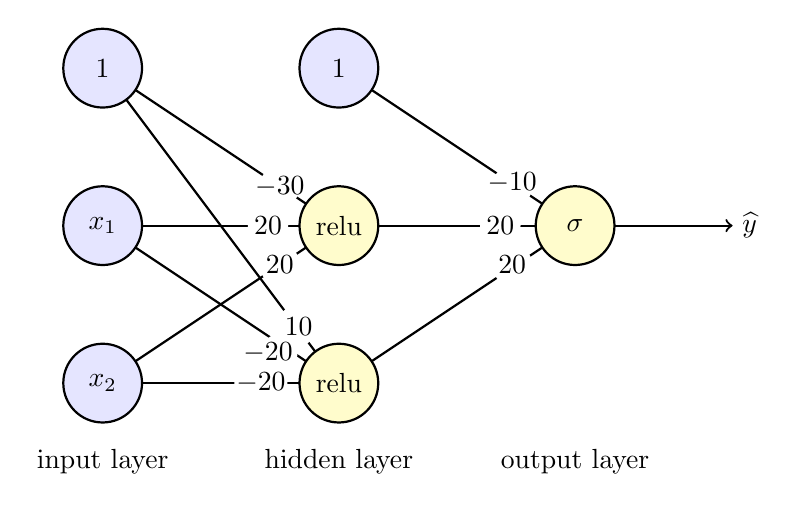
\begin{tikzpicture}

        \draw[thick] (-2, 2) -- (1, 0);
        \draw[thick] (-2, 2) -- (1, -2);
        \draw[thick] (-2, 0) -- (1, 0);
        \draw[thick] (-2, 0) -- (1, -2);
        \draw[thick] (-2, -2) -- (1, 0);
        \draw[thick] (-2, -2) -- (1, -2);

        \draw[thick] (1, 2) -- (4, 0);
        \draw[thick] (1, 0) -- (4, 0);
        \draw[thick] (1, -2) -- (4, 0);

        \draw[thick, ->] (4, 0) -- (6, 0);

        \draw[fill=white, white] ({-2 + \qq*3}, {2 - \qq*2}) circle (0.25);
        \node at ({-2 + \qq*3}, {2 - \qq*2}) {$-30$};

        \draw[fill=white, white] ({-2 + \rr*3}, 0) circle (0.25);
        \node at ({-2 + \rr*3}, 0) {$20$};

        \draw[fill=white, white] ({-2 + \qq*3}, {-2 + \qq*2}) circle (0.25);
        \node at ({-2 + \qq*3}, {-2 + \qq*2}) {$20$};

        % \node at (0.5, 0.6) {$-30$};
        % \node at (0.25, 0.2) {$20$};
        % \node at (0.25, -0.25) {$20$};

        % \node at (0.75, -1.25) {$10$};
        % \node at (0.1, -1.77) {$-20$};
        % \node at (0.1, -2.2) {$-20$};

        \draw[fill=white, white] ({-2 + 0.82*3}, {2 - 0.82*4}) circle (0.25);
        \node at ({-2 + 0.83*3}, {2 - 0.82*4}) {$10$};

        \draw[fill=white, white] ({-2 + 0.67*3}, -2) circle (0.33);
        \node at ({-2 + 0.67*3}, -2) {$-20$};

        \draw[fill=white, white] ({-2 + \qq*3}, {- 0.8*2}) circle (0.22);
        \node at ({-2 + 0.7*3}, {-0.81*2}) {$-20$};

        \draw[fill=white, white] (3.2, 0.5) circle (0.25);
        \node at (3.2, 0.55) {$-10$};

        \draw[fill=white, white] (3.05, 0) circle (0.25);
        \node at (3.05, 0) {$20$};

        \draw[fill=white, white] (3.2, -0.5) circle (0.25);
        \node at (3.2, -0.5) {$20$};



        \draw[thick, fill=blue!10] (-2, 2) node {$1$} circle (0.5);
        \draw[thick, fill=blue!10] (-2, 0) node {$x_1$} circle (0.5);
        \draw[thick, fill=blue!10] (-2, -2) node {$x_2$} circle (0.5);

        \draw[thick, fill=blue!10] (1, 2) node {$1$} circle (0.5);
        \draw[thick, fill=yellow!20] (1, 0) circle (0.5);
        \node at (1, 0) {relu};
        \draw[thick, fill=yellow!20] (1, -2) circle (0.5);
        \node at (1, -2) {relu};

        \draw[thick, fill=yellow!20] (4, 0) circle (0.5);
        \node at (4, 0) {$\sigma$};

        \node[right] at (6, 0) {$\widehat{y}$};

        \node at (-2, -3) {input layer};
        \node at (1, -3) {hidden layer};
        \node at (4, -3) {output layer};
        

        % \node[right] at (4.5, 0) {$\hat y =\displaystyle{\begin{cases}0&\text{if $a_1^{[1]}\leq 1/2$}\\[1ex]1&\text{if $a_1^{[1]}> 1/2$}\end{cases}}$};
    \end{tikzpicture}
\end{document}